% *******************************************************************************
% * Copyright (c) 2007-2008 by Elexis
% * All rights reserved. This document and the accompanying materials
% * are made available under the terms of the Eclipse Public License v1.0
% * which accompanies this distribution, and is available at
% * http://www.eclipse.org/legal/epl-v10.html
% *
% * Contributors:
% *    G. Weirich
% *
% *  $Id: konzepte.tex 5231 2009-04-02 13:16:56Z rgw_ch $
% *******************************************************************************
% !Mode:: "TeX:UTF-8" (encoding info for WinEdt)

\section{Contacts}
\label{kontakt}
\index{contact!définition}
Dans Elexis, chaque personne ou entreprise qui est dans une relation avec le cabinet, est
tout d'abord un\glqq contact\grqq{}. La saisie ou la modification des contacts se fait dans la perspective de contact.
\begin{flushleft}
    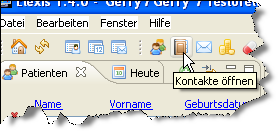
\includegraphics{images/contactperspective}
\end{flushleft}


Ils existent les types de contact suivants :
\begin{itemize}
  \item personne
	\begin{itemize}
  		\item mandant
  		\item utilisateur
  		\item patient
  		\item autres
    \end{itemize}
    \item{oganisation}
    \begin{itemize}
      \item{laboratoire}
      \item {autres}
    \end{itemize}
\end{itemize}


\section{Utilisateurs et Mandants}
\index{utilisateur!définition}\index{mandant!défintion}
Quelqu'un qui a le droit de facturer ses prestations à charge de l'assurance obligatoire de soins (ce qui est en Suisse seulement possible si on a son propre numéro de concordat RCC ), est un \textit{mandant}. Chaque processus dans Elexis (consultation, laboratoire, prescription etc.) se passe toujours sous la responsabilité et sur le compte précisément d'un Mandant. \index{mandant}

\medskip

JQuelqu'un qui peut manier le programme , est un \textit{utilisateur}. Un utilisateur travaille toujours sur ordre d'un Mandant spécifique.

Ainsi il existe à chaque moment dans Elexis un Mandant actuel et un utilisateur actuel.
\index{utilisateur}Mandant und Anwender können auch identisch sein (Wenn der
Mandant selbst am PC arbeitet).
Le Mandant et l'utilisateur peut aussi être identique (si le Mandant lui-même travaille au PC). Un utilisateur peut aussi modifier l'attribution à un Mandant (si une assistante médicale dans un cabinet de groupe travaille par exemple pour des Mandants différentes).
\index{groupes}\index{droits}
\index{droits}\index{utilisateur!droits}
Des utilisateurs ont certains droits individuellement réglables, avec lesquels on peut contrôler très finement à qui on permet quelles actions dans Elexis. Des utilisateurs peuvent aussi être rassemblés dans des groupes qui définissent certains droits communs (p. ex. groupes  \glqq assistantes médicales\grqq{} ou \glqq médecins\grqq{}). Le groupe \glqq Admin\grqq{}: est un groupe spécial : Celui qui fait partie de ce groupe, a automatiquement  \textit{tous} les droits.

\medskip

\textbf{Important}: Même si cela peut d'abord vous apparaître illogique : Aussi le chef ne devrait pas travailler habituellement comme Admin \index{administrateur}.
La raison se trouve dans le fait que l'Admin-Account permet aussi des suppressions irréversibles et d'autres modifications très désagréables. Dans l'état fiévreux du quotidien on risque facilement de cliquer une fois sur le faux bouton !
Par conséquent : Travaillez dans le quotidien avec un Account qui donne précisément les droits dont vous avez besoin au quotidien. Etablissez un deuxième Account pour vous,celui qu'est assigné au groupe Admin, et ne vous annoncez sous cet Account que lorsqu'il est vraiment nécessaire.

Le concept des groupes et droits est expliqué plus précisément à partir de la page\pageref{sec:gruppen} .

\section{Consultations, cas, garants et répondant des coûts}
\index{consultation!définition}\index{cas!définition}\index{facturation} Chaque contact retenu dans les Elexis entre le personnel du cabinet et un patient est une  \textit{consultation}. Lorsqu'une consultation est comptabilisé la facturation sera faite en faveur du Mandant, pour lequel l'utilisateur connecté a travaillé.
\label{definition:fall}
Chaque consultation est aussi assignée à un \textit{cas}. Ein Fall ist hier eher eine versicherungstechnische, als eine medizinische Einheit: Un cas est ici plutôt une entité assécurologique qu'une entité médicale : Le cas rassemble toutes les consultations qui sont comptabilisées avec le même système de facturation (voir\ref{settings:abrechnungssystem}à la page \pageref{settings:abrechnungssystem}). Cela peut parfois être identique avec la notion de cas médical (un accident qui est facturé à un assureur spécifique avec un numéro de cas spécifique), ou ne peut pas avoir de lien avec un cas médical  (p. ex. en général en Suisse un cas de maladie sera subsumé à la \glqq maladie\grqq{} qui rassemble toutes les consultations LAMAL).

Un cas ne peut être attribué à qu'un seul patient et un système, mais peut toutefois comprendre des consultations de plusieurs Mandants. (Une facture distincte est alors fournie pour chaque Mandant).

\section{Sticker}
\index{stickers}\index{étiquettes}\index{marquage}
\label{Etiketten}
Des patients et d'autres contenus de base de données peuvent être marqués avec des 'stickers' (étiquettes). Un 'sticker' est une caractéristique en principe arbitraire qui est liée avec un objet correspondant de la base de données. Par exemple un patient pourraient être marqué avec le 'sticker' 'modèle de médecin de famille', 'MRSA' ou autre. Un tel 'sticker' est affichée lors de l'appel de l'objet correspondant.

 Des 'stickers' sont définis sous \textsc{Fichier-Paramètres-Sticker} (page Fig. \ref{fig:etiketten1}). ELa quantité des stickers peut être définie au choix. Pour créer un nouveau sticker, écrivez le texte pour le sticker dans le champ en haut et cliquez sur 'nouveau sticker'. Le 'sticker' que vous venez de créer apparaît alors avec des valeurs standards sur la liste des stickers. Sélectionnez le sticker et suggérez une image (format 16x16 tout au plus à 32x32 pixels), une couleur de texte et une couleur d'arrière-plan.
L'importance de la  'valeur' vous est expliquée ci- dessous.


\begin{figure}
    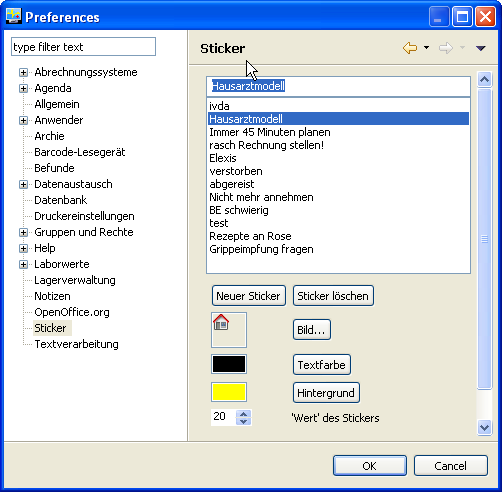
\includegraphics{images/etikette1}
    \caption{Sticker erstellen}
    \label{fig:etiketten1}
\end{figure}

Des stickers crées de cette façon peuvent être attribués à un patient qui se trouve sur la liste des patients par un clic sur la touche droite de la souris ce qui permet de choisir un 'Sticker' sur un menu déroulant. On peut attribuer à chaque patient entre zéro et x 'stickers'. On trouvera dans la liste des patients la saisie correspondante avec les 'stickers' et images, couleur du texte et couleur d'arrière plan.  (Fig. \ref{fig:etiketten2}).
\begin{figure}
    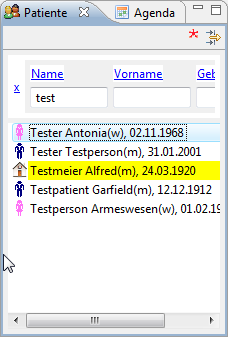
\includegraphics{images/etikette3}
    \caption{Anzeige der Sticker}
    \label{fig:etiketten2}
\end{figure}

Ici, on voit alors aussi le sens de l'attribut 'valeur' d'un sticker:
Lorsqu'un patient a reçu plusieurs stickers assignés, la liste des patients indique toujours
celui avec  'la valeur' la plus élevée. Les chiffres que vous utilisez là concrètement n'ont pas d'importance car la valeur absolue ne joue pas de rôle, par contre les relations entre les 'valeurs'.


\medskip

Si vous ouvrez une consultation pour y faire vos notes, vous y voyez toutes les stickers assignées au patient.
\begin{figure}
    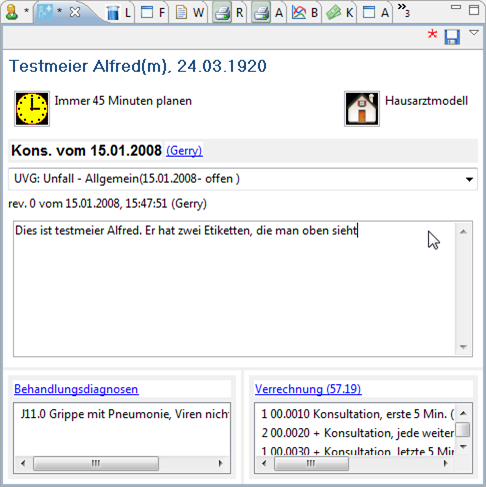
\includegraphics{images/etikette2}
    \caption{Konsultation mit Stickern}
    \label{fig:etiketten3}
\end{figure}


\clearpage

\section{Décompte des prestations}
\label{concept:leistung}
\index{Codes de prestation}\index{faire les comptes}
\begin{wrapfigure}{l}{7.5cm}
    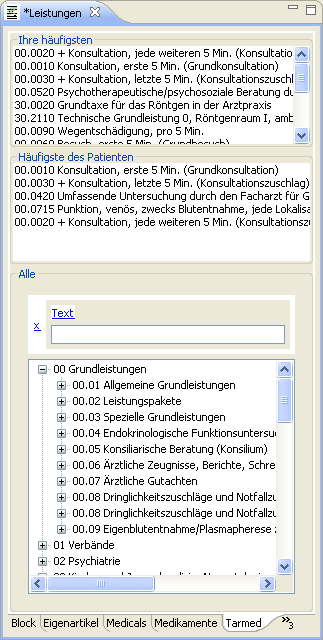
\includegraphics[width=7.5cm]{images/leistungen1}
    \caption{Leistungen}
    \label{fig:leistungen}
\end{wrapfigure}
\index{prestation!comptabiliser}
Les codes de prestations qui peuvent être comptabilisé, sont fournis d'une part par les Plugins (p. ex. par Elexis-tarif médical-Suisse), d'autre part par des blocs de prestations définis par vous-même (voir ci-dessous).
Vous trouvez tous les systèmes de codage de prestations existants sous la fenêtre
\glqq prestations\grqq{} (Fig. \ref{fig:leistungen}): Vous voyez au bord inférieur de la fenêtre un onglet pour chaque système de codage installé. 
Cette fenêtre apparaît lorsque vous cliquez depuis la fenêtre de consultation sur
 \glqq{}saisie prestations\grqq{}. La structure est la même pour chaque système de codage de prestations :

La fenêtre partielle supérieure montre les codes les plus fréquemment appliqués par vous dans ce système de codage de prestations, chose qui vous permet un accès rapide sans chercher longtemps. La liste est mise à jour régulièrement et plus vous utilisez un certain code, plus haut dans la liste il apparaîtra lors de la prochaine ouverture de la fenêtre.


\medskip
Dans la partie moyenne, les codes jusqu'ici utilisés les plus fréquemment pour ce patient apparaissent triés selon
le même principe. La fenêtre partielle la plus basse met à disposition le système de codage de prestation entier
avec toute sa systématique.


\bigskip

Pour introduire un code de prestation, vous pouvez le tirer d'une des trois sections de la fenêtre de 'prestations' dans la fenêtre de 'saisie prestations' ou le choisir par double-clic.
Certains Plugins peuvent contenir un  \glqq Optifier\grqq (Optimizer/Verifier) qui reconnaît des erreurs et/ou peut appliquer des corrections. Ainsi refuse par exemple le Tarmed- Plugin d'une part la facturation double du code \textit{00.0010 Consultation 5 premières minutes } avec un message d'erreur  (Verifier), et d'autre part il ajoute automatiquement le code 00.0010 lorsque vous introduisez le code 00.0030 \textit{00.0030 Consultation 5 dernières minutes} car 00.0030 se combine toujours avec 00.0010 (Optimizer).
Les\textit{articles}, qui sont remis directement au patient peuvent aussi être comptabilisés directement depuis cette fenêtre et leur stock est automatiquement ajusté.

\subsection{Blocs de prestations et prestations propres}
\begin{wrapfigure}{r}{6cm}
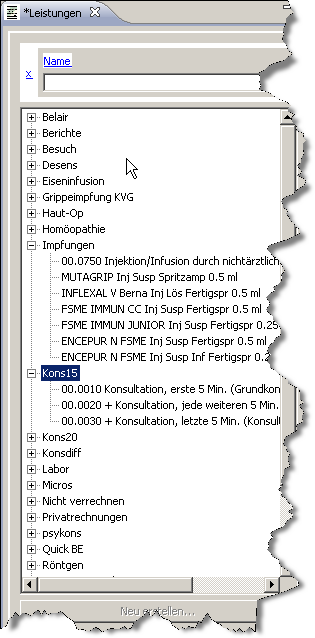
\includegraphics{images/block1}
\caption{Leistungsblöcke}
\label{fig:bloecke}
\end{wrapfigure}
\index{prestations propres}
\index{blocs de prestations}
Comme autre allègement du travail Elexis permet aussi de résumer plusieurs codes de prestation dans des blocs de prestation qui seront comptabilisé entièrement ou partiellement, et ceci même si ces blocs proviennent des systèmes de codage de prestation tout à fait différents. A part des blocs de prestations de provenance des systèmes de codage de prestations pré installés, de tels blocs peuvent contenir aussi des éléments à comptabiliser définis par vous même.
Vous voyez dans la Fig.\ref{fig:bloecke} quelques exemples :\textit{cons15} est un exemple de bloc qui est comptabilisé
généralement en bloc. Pour ce faire vous pouvez, tirer le bloc avec la souris dans la fenêtre de saisie de prestation de la consultation ou, si vous travaillez plutôt avec le clavier, vous tapez le nom du bloc, suivi de la clé de libération des macros dans le texte de consultation
(conformément aux normes c'est le \#). L'entrée de cons15\# dans le texte de consultation comptabiliserait ainsi dans notre exemple une consultation de 15-minutes selon tarif Tarmed.
\textit{Les Vaccinations} seraient un exemple de bloc, qui serait plutôt pensé comme sommaire d'éléments semblables
(avec le but d'un gain de temps pour trouver plus rapidement l'élément cherché) qui seront de toute façon comptabilisé
séparément. Dans ce cas, on tire simplement les différents éléments du bloc dans la fenêtre de saisie de prestation .


Pour créer un nouveau bloc, on introduit (à libre choix mais toutefois unique) un nom pour ce bloc et clique ensuite sur \textit{créer nouveau ...}. Les prestations s'ajoutent au bloc dans la fenêtre des codes(voir  Fig. ref{fig:bloecke2}).
\begin{figure}[htp]
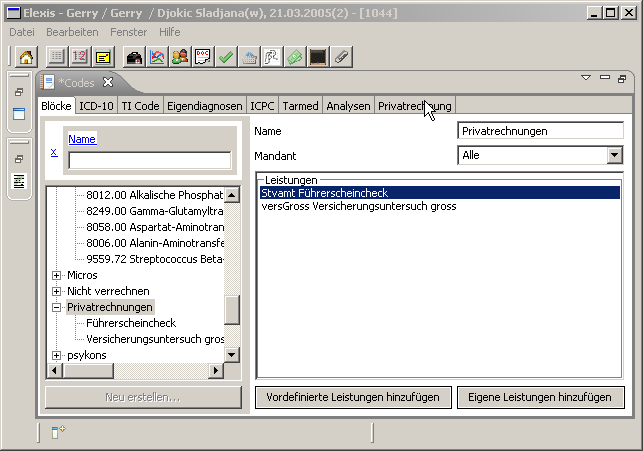
\includegraphics[width=0.9\textwidth]{images/block2}
\caption{Leistungsblock definieren}
\label{fig:bloecke2}
\end{figure}
Vous pouvez ajouter par drag\&drop soit des prestations prédéfinies de provenance d'un des systèmes de code installés, soit définir vos propres prestations. Ici vous devez aussi indiquer frais et prix en centimes/cents ainsi que le temps budgétisé pour la prestation en minutes.


\section{Articles et stocks}
\index{article}\index{médicament}\index{stock}
 Tout ce qui peut être acheté, stocké, livré ou prescrit est un  \textit{article}.
 Les articles sont organisés dans des classes par exemples classes au \textit{médicaments},
 ou à des  \textit{LiMA} ou au\textit{matériel bureautique}.
 Elexis peut adopter chaque article qui lui est connu comme \textit{article en stock}.

 Un article en stock est un article dont l'existence est contrôlée et qui peut être commandé si nécessaire de façon semi-automatique. Des plus amples informations concernant les articles et leur stockage se trouvent dans la description de la View (à la page \pageref{view:artikel} et suivantes.)

\section{Importation des données externes }
\index{importation}
En principe Elexis est en mesure d'importer des données de n'importe quelle source .
Toutefois, le format de ces données doit naturellement être connu ou standardisé d'une certaine manière. Par conséquent l'importation de données est en générale effectué par les 'Importer-Plugins'.
Il y existent des 'Importers' pour des données d'annuaire téléphonique, pour les bases de données d'autres programmes pour le cabinet médical, pour des laboratoires externes, pour des appareils de laboratoire et pour d'autres appareils médicaux qui sont capables de transférer leurs données sur un ordinateur, pour des LiMA, des médicaments,
le Tarmed et d'autres bases de données etc.
Vous trouvez une liste de Plugins disponibles dans le menu 'Plugins' sur  http://www.elexis.ch. Des 'Importers' supplémentaires peuvent être programmés assez facilement, en cas de besoin vous pouvez nous contacter pour demander un devis.

\medskip

Les 'Importers' se trouvent généralement dans le menu local des 'Views' qui affichent les données correspondantes (p. ex. Tarmed-Importer ou Importer du laboratoire). Une classe d' 'Importers' qui ne sont pas attribués à certaine 'View' se trouvent aussi dans le menu d' 'importation de données' sous 'Fichier' dans la barre de menu. Ici, un dialogue s'ouvre comme dans la fig. \ref{fig:importdlg}.
\begin{figure}
  % Requires \usepackage{graphicx}
  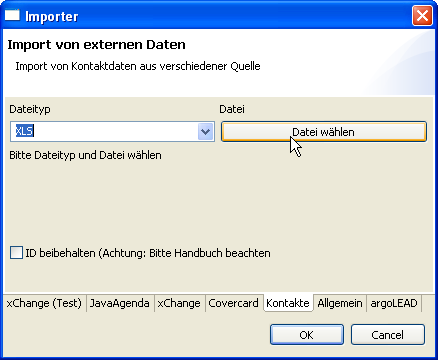
\includegraphics{images/importdlg}\\
  \caption{Import-Dialog}\label{fig:importdlg}
\end{figure}
\index{Import!contacts}
Dans les onglets en bas de la fenêtre vous trouvez tous les 'Importers' de base installés. Lesquels s'y trouvent dépend des Plugins installés. Seulement le 'Contact-Importer' qui est choisi dans l'illustration existe toujours. Cet 'Importer' peut importer des contacts des fichiers externes, pour autant que ceux-ci soient préparés de façon standardisée en forme de tableaux. Choisissez sous 'le type de fichiers' s'il s'agit d'un tableau Microsoft\texttrademark Excel\texttrademark(xls), d'un tableau Caracter Separated Values (csv) ou d'un tableau de Santésuisse contenant les assureurs et leurs codes EAN.
S'il s'agit de xls, le fichier doit contenir un tableau 0 avec les colonnes suivantes :


\begin{tabular}[h]{|l|l|}
\hline Titre de colonne & Légende\\
\hline
\hline  ID & une identification (en principe au choix mais univoque dans le fichier)\\
\hline Istpersonne & 1 si la saisie concerne une personne, 0 pour tout les autres cas (organisations etc)\\
\hline Istpatient & 1 si la saisie concerne un patient, 0 pour tout les autres cas\\
\hline titre & titre, personne de référence etc.\\
\hline désignation1 & En cas d'une personne son nom de famille\\
\hline désignation2 & En cas d'une personne son prénom\\
\hline supplément & \\
\hline date de naissance & En format dd.mm.yyyy ou yyyy-mm-dd\\
\hline genre & m ou f ou un mot qui commence avec m ou f\\
\hline e-Mail & adresse E-Mail\\
\hline website & une adresse WWW\\
\hline téléphone 1 & Numéro de téléphone primaire\\
\hline téléphone 2 & Numéro de téléphone supplémentaire\\
\hline mobil & Numéro de téléphone portable\\
\hline rue & Rue et numéro de maison\\
\hline code postal & code postal écrit comme 1224 ou comme CH-1224 (doit être formaté comme fichier texte)\\
\hline localité & \\
\hline adresse & Adresse comme elle apparaîtra sur une étiquette d'adresse. Nouvelle ligne par $\backslash$n\\
\hline EAN & Code EAN comme EAN13\\
\hline
\end{tabular}

\medskip

Pour que le format puisse être reconnu la première ligne du tableau doit contenir les titres de colonne précisément dans la forme de présentation ci-dessus. Chacune des colonnes citées doit exister mais peut toutefois être vide. Le fichier doit donc être codé comme iso-8859-1 (c'est une norme sous Windows ; avec la version MAC de Excel, le codage d'exportation devrait en conséquence éventuellement être adapté).


\medskip

Si vous avez fixé le type de fichier, cliquez vous sur le bouton 'choisir fichier' et cherchez le fichier à importer. Ne placez un crochet à 'préserver ID' seulement 
 \textbf{seulement},lorsque \begin{itemize}
\item chaque paquet de données dans le champ ID a une ID 
\item cette ID est univoque, et ne peut donc entrer en collision avec aucun autre contact dans Elexis
\item il est indispensable de maintenir cette ID.
\end{itemize}
Si vous ne placez pas le crochet, chose qui est recommandée dans la plupart des cas, alors Elexis fournira lors de l'importation une identité univoque pour chaque contact (comme si on introduisait manuellement ce contact).\\
Cliquez alors OK, pour commencer l'importation.

 \section{Plusieurs instances simultanément}
 \index{simultanément}
 Vous pouvez démarrer Elexis sans problèmes plusieurs fois simultanément pour afficher dans les fenêtres des perspectives différentes ou différents patients.
Certains éléments peuvent aussi être échangés par Cut\&Paste entre les instances courantes. Exemples d'application :

 \begin{itemize}
   \item Vous travaillez sur une entrée de patient et vous recevez un appel téléphonique  concernant un autre patient. Au lieu de quitter votre travail vous cliquez sur l'Elexis qui est ouvert en arrière plan et cherchez le dossier de ce patient.
   \item A son poste de travail votre assistante médicale voudrait avoir en même temps l'agenda et les données des patients à portée de vue. Si vous lui payez un deuxième écran (au lieu d'un deuxième PC), vous attachez les deux écrans au même PC à une carte graphique DualHead et mettez sur chaque écran une instance propre de Elexis.
   \item Pendant que l'Elexis est occupé à faire la facturation qui prend du temps, vous ne voudriez pas glander. Sans problème, vous démarrez une deuxième instance d'Elexis et continuez à travailler. (Vous pourriez naturellement aussi aller boire un café ou faire une promenade).
   \item Vous écrivez une lettre, mais vous aimerez y mettre certaines parties d'une autre lettre.
Ouvrez dans une instance d'Elexis l'ancienne lettre, copiez là certains passages et collez les dans l'autre lettre que vous êtes en train d'écrire dans l'autre instance d'Elexis.

 \end{itemize}

\section{Plugins}
\index{Plugin!définition}
Ce concept est discuté en détail à la page \pageref{expl:plugins}. Ici mentionnons pour le moment seulement : Elexis est extensible dans tout les sens. Il n'y a pas seulement un certain nombre de \glqq modules\grqq{} mais en fait, à tout moment, des nouvelles fonctions peuvent être programmé dont lors du lancement de la version actuelle on n'avait pas encore connaissance. Cela se fait sous forme de \glqq Plugins\grqq{}. Les 'plugins' peuvent être programmés par exemple pour, de la statistique, la comptabilité, l'importation de données de laboratoire, l'accessibilité des
appareils, l'exportation des données du dossier médical, des nouveaux systèmes de comptabilisation des prestations, des nouveaux systèmes de classifications des diagnostics etc.
Donc un 'Plugin' est dans Elexis simplement un programme avec des capacités au choix qui a la propriété de pouvoir coopérer avec Elexis.
Il est impossible de présenter ni dans ce guide ni ailleurs une liste exhaustive de tous les 'Plugins' parce que personne ne peut savoir quels 'Plugins' ont été commandés par des usagers indépendants auprès des programmeurs indépendants.
Un listing de tout les 'Plugins' qui nous sont connus se trouve sur : http://www.elexis.ch



